\subsubsection{Quản lý phân quyền (RBAC)}
\begin{figure}[H]
    \centering
    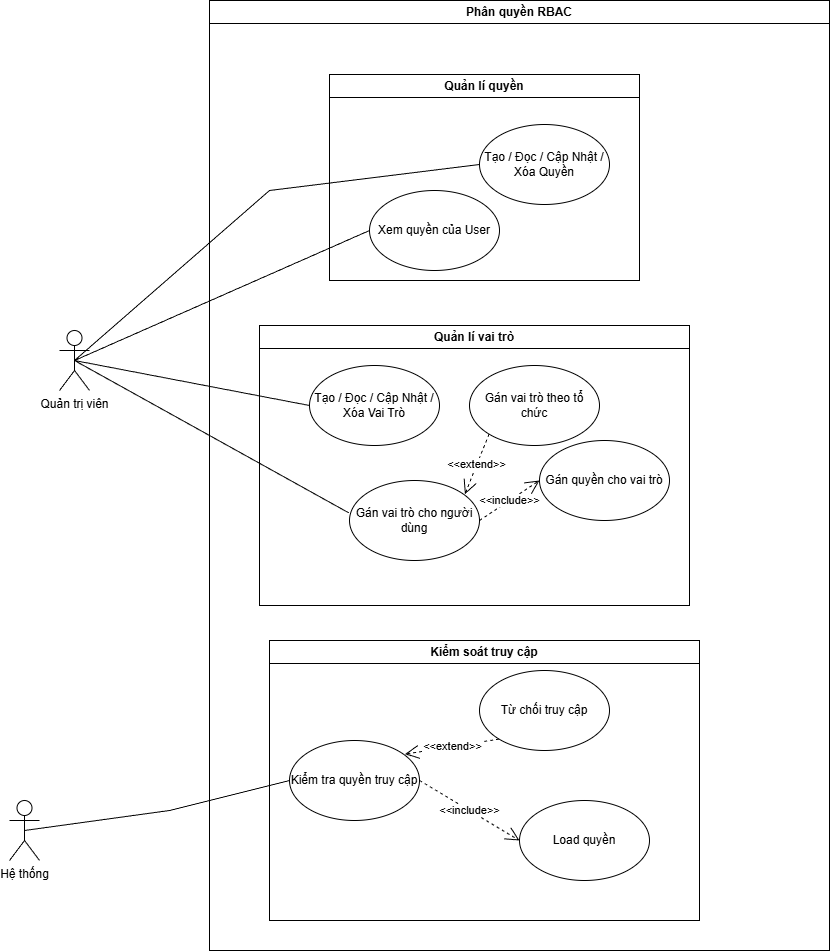
\includegraphics[width=1.0\linewidth]{Images/use-case-diagram/UC05_authorization-usecase.drawio.png}
    \vspace{0.3em}
    \caption{UC05 -  Gán vai trò và Phân quyền}
    \label{fig:uc01-usecase}
\end{figure}
\renewcommand{\arraystretch}{1.3}
\begin{longtable}{|m{0.25\textwidth}|m{0.75\textwidth}|}
\hline

\textbf{Use-case Name} & \textbf{UC05. Gán vai trò và Phân quyền} \\ \hline
\endfirsthead

\hline
\textbf{Use-case Name (tiếp)} & \textbf{UC05. Gán vai trò và Phân quyền} \\ \hline
\endhead

% ===== Nội dung bảng =====
\textbf{Actors} 
& \begin{itemize}[label=--]
    \item Quản trị viên (Admin)
    \item Hệ thống (System)
\end{itemize} \\ 
\hline

\textbf{Description} 
& Quản trị viên thực hiện cấp quyền cho người dùng bằng cách gán các vai trò (Roles) cụ thể. 
Hệ thống sẽ tự động liên kết các quyền hạn (Permissions) tương ứng với vai trò đó. Ngoài ra, hệ thống hỗ trợ việc gán vai trò trong phạm vi một tổ chức/đơn vị cụ thể nếu cần thiết. \\ 
\hline

\textbf{Trigger} 
& Quản trị viên chọn một tài khoản người dùng và nhấn nút truy cập vào màn hình "Chọn vai trò vai trò". \\ 
\hline

\textbf{Pre-Conditions} 
&
\begin{itemize}[label=--]
    \item Quản trị viên đã đăng nhập và có quyền quản lý hệ thống.
    \item Các Quyền (Permissions) đã được định nghĩa trong cơ sở dữ liệu.
    \item Tài khoản người dùng cần gán đã tồn tại.
\end{itemize}
\\ 
\hline

\textbf{Post-Conditions} 
&
\begin{itemize}[label=--]
    \item Người dùng được cập nhật vai trò mới và có các quyền truy cập tương ứng.
    \item Thông tin phân quyền được lưu vào cơ sở dữ liệu.
\end{itemize}
\\ 
\hline

\textbf{Normal Flow} 
&
\begin{enumerate}
    \item Quản trị viên tìm kiếm và chọn người dùng cần phân quyền.
    \item Hệ thống hiển thị danh sách các Vai trò khả dụng (Ví dụ: Admin, Mod, User...).
    \item Quản trị viên chọn vai trò muốn gán cho người dùng.
    \item \textbf{(Include)} Hệ thống thực hiện quy trình \textit{"Gán quyền cho vai trò"}: Tự động ánh xạ các quyền hạn (Create/Read/Update/Delete) đi kèm với vai trò đã chọn.
    \item Quản trị viên xác nhận lưu thay đổi.
    \item Hệ thống cập nhật dữ liệu và thông báo thành công.
\end{enumerate}
\\ 
\hline

\textbf{Alternative Flow} 
& Tại bước 3 (Trường hợp gán theo phạm vi tổ chức):
\begin{itemize}
    \item \textbf{3a.} Nếu vai trò yêu cầu phạm vi cụ thể (ví dụ: Bí thư của tổ chức A), Quản trị viên chọn thêm thông tin Tổ chức/Đơn vị.
    \item \textbf{3b.} \textbf{(Extend)} Hệ thống kích hoạt quy trình \textit{"Gán vai trò theo tổ chức"} để kiểm tra và giới hạn phạm vi quyền hạn trong tổ chức đó.
    \item \textbf{3c.} Tiếp tục sang bước 4.
\end{itemize}
\\ 
\hline

\textbf{Exception} 
& Tại bước 6:
\begin{itemize}
    \item \textbf{6a.} Hệ thống gặp lỗi kết nối cơ sở dữ liệu. Hiển thị thông báo: \textit{"Lưu thất bại, vui lòng thử lại sau."}
    \item \textbf{6b.} Tài khoản người dùng đang bị khóa hoặc không hợp lệ. Hệ thống từ chối phân quyền và báo lỗi.
\end{itemize}
\\
\hline
\caption{Bảng mô tả Use Case UC05 - Gán vai trò và Phân quyền}
\end{longtable}